\begin{note}
    此小节还未完成。
\end{note}

\subsection{滤波器的表示}

\begin{definition}
    \bd{滤波器}是以特定方式改变信号的频率特性,从而变换信号的处理系统。
    滤波器一般有如下类别,如图 \ref{fig:filter_types} 所示:
    \begin{enumerate}[label=(\arabic*)]
        \item 高通滤波器(HP)
        \item 低通滤波器(LP)
        \item 带通滤波器(BP)
        \item 带阻滤波器(BS)
        \item 全通滤波器(AP)
    \end{enumerate}
    \begin{figure}[H]
        \centering
        \includegraphics[width=0.8\textwidth]{chap4/img/filter_types.png}
        \caption{滤波器类型}
        \label{fig:filter_types}
    \end{figure}

    滤波器也可以被分为\bd{模拟滤波器}和\bd{数字滤波器}。
    \begin{itemize}
        \item \bd{模拟滤波器}是由电阻、电容、电感等部件构成的电路。
            滤波器特性对所用部件的物理标称值非常敏感,而且,
            有些部件的物理特性会随温度变化而改变。
        \item \bd{数字滤波器}是用软件实现的,很少依赖硬件。滤波软件
            只是一系列程序指令。虽然它是在硬件平台上运行,但
            是硬件平台本身并不决定滤波器的性能。数字滤波器的
            性能是由\bd{一组系数}确定的。
    \end{itemize}
    数字滤波器的实现方式一般有以下几种:
    \begin{enumerate}
        \item 用流图计算滤波器的输出。
        \item 用差分方程计算滤波器的输出。
        \item 用卷积过程计算滤波器的输出。
        \item 用 DTFT 直接改变信号频谱。
    \end{enumerate}
\end{definition}

\begin{definition}
    模拟
\end{definition}

\begin{example}
    \label{exercise:serial-flow-graph}
    写出如图 \ref{fig:serial-flow-graph} 所示级联流图的差分方程。
    \begin{figure}[H]
        \centering
        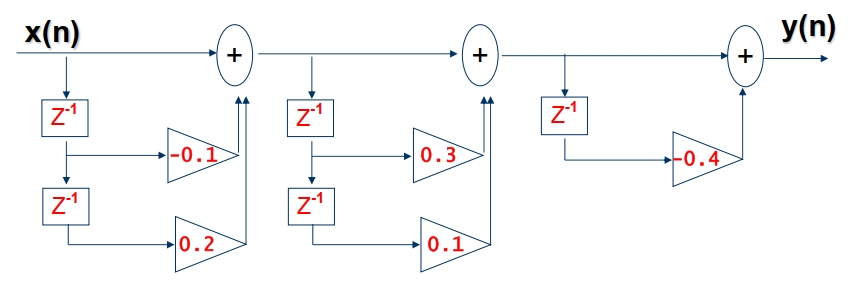
\includegraphics[width=0.8\textwidth]{chap4/img/serial_flow_graph.png}
        \caption{例 \theexample~ 的级联流图}
        \label{fig:serial-flow-graph}
    \end{figure}
\end{example}

\begin{solution}
    不妨设 $x(n) = x_1(n), y(n) = y_3(n)$,
    以及 $y_1(n) = x_2(n), y_2(n) = x_3(n)$,则如图 \ref{fig:serial-flow-graph-annotated} 所示,
    \begin{align*}
        y_1(n) & = x_1(n) - 0.1x_1(n - 1) + 0.2x_1(n - 2), \\
        y_2(n) & = x_2(n) + 0.3x_2(n - 1) + 0.1x_2(n - 2), \\
        y_3(n) & = x_3(n) - 0.4x_3(n - 1).
    \end{align*}
    \begin{figure}[H]
        \centering
        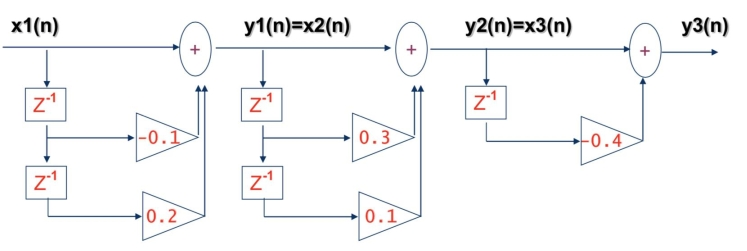
\includegraphics[width=0.8\textwidth]{chap4/img/serial_flow_graph_annotated.png}
        \caption{例 \theexample~ 的级联流图(带标注)}
        \label{fig:serial-flow-graph-annotated}
    \end{figure}
    将 $y_1(n)$ 代入 $y_2(n)$ 的表达式中,将 $y_2(n)$ 代入 $y_3(n)$ 的表达式中,
    可得级联流图的差分方程为
    \begin{align*}
        y_3(n) = x_1(n) - 0.2x_1(n - 1) + 0.19x_1(n - 2) - 0.058x_1(n - 3) - 0.008x_1(n - 5).
    \end{align*}
\end{solution}

\begin{exercise}
    \label{exercise:LTI-stable}
    证明:某 LTI 系统稳定的充要条件是
    \begin{align*}
        \sum_{n = -\infty}^{\infty} |h(n)| = P < \infty.
    \end{align*}
    其中 $h(n)$ 为系统的单位脉冲响应,$P$ 为一个常数。
\end{exercise}

\begin{homework}
    已知某系统的差分方程如下式:
    \begin{align*}
        y(n) = x(n) + x(n - 3) + 0.7y(n - 1) + 0.6y(n - 2).
    \end{align*}
    \begin{enumerate}[label=(\arabic*)]
        \item 判断系统的脉冲响应类型。
        \item 画出该系统的信号流图。
    \end{enumerate}
\end{homework}

\begin{solution}
    \begin{enumerate}[label=(\arabic*)]
        \item 该系统的脉冲响应类型为无限脉冲响应。
        \item 该系统的直接 I 型信号流图如图 \ref{fig:signal_flow_diagram} 所示。
        \begin{figure}[H]
            \centering
            \tikzstyle{block} = [draw, rectangle, minimum height=1cm, minimum width=1cm]
            \tikzstyle{circ} = [draw, fill, circle, inner sep=1.5pt]
            \tikzstyle{no-circ} = [draw, circle, inner sep=0pt]
            \tikzstyle{sum} = [draw, circle]
            \tikzstyle{line} = [draw, -latex]
            \tikzstyle{no-arrow-line} = [draw, -]
            \tikzstyle{gainx} = [draw, isosceles triangle, isosceles triangle apex angle=60]
            \tikzstyle{gainy} = [draw, isosceles triangle, isosceles triangle apex angle=60, shape border rotate=180]
            \begin{tikzpicture}
                \node [name=input] (input) {$x(n)$};
                \node [circ, right of=input, xshift=1cm] (circx) {};
                \path [no-arrow-line] (input) -- (circx);
                \node [sum, right of=circx, xshift=4cm] (sum) {$+$};
                \node [circ, right of=sum, xshift=4cm] (circy) {};
                \path [no-arrow-line] (sum) -- (circy);
                \node [name=output, right of=circy, xshift=1cm] (output) {$y(n)$};
                \path [line] (circy) -- (output);
        
                \node [block, below of=circx, yshift=-1cm] (zx1) {$Z^{-1}$};
                \path [line] (circx) -- (zx1);
                \node [block, below of=zx1, yshift=-2cm] (zx2) {$Z^{-1}$};
                \path [line] (zx1) -- (zx2);
                \node [block, below of=zx2, yshift=-2cm] (zx3) {$Z^{-1}$};
                \path [line] (zx2) -- (zx3);
        
                \node [block, below of=circy, yshift=-1cm] (zy1) {$Z^{-1}$};
                \path [line] (circy) -- (zy1);
                \node [block, below of=zy1, yshift=-2cm] (zy2) {$Z^{-1}$};
                \path [line] (zy1) -- (zy2);
        
                \path [line] (circx) -- (sum);
                \coordinate (zgx3) at ([xshift=2cm, yshift=-1cm] zx3);
                \path [no-arrow-line] (zx3) |- (zgx3);
                \path [line] (zgx3) -- (sum);
                \node [gainy, below of=zy1, xshift=-2cm, yshift=-0.5cm] (zgy1) {$0.7$};
                \node [circ, below of=zy1, yshift=-0.5cm] (circy1) {};
                \path [line] (circy1) -- (zgy1);
                \path [line] (zgy1.west) -- (sum);
                \node [gainy, below of=zy2, xshift=-2cm, yshift=-0.5cm] (zgy2) {$0.6$};
                \path [line] (zy2) |- (zgy2);
                \path [line] (zgy2.west) -- (sum);
            \end{tikzpicture}
            \caption{作业 \thehomework~ 的信号流图}
            \label{fig:signal_flow_diagram}
        \end{figure}
    \end{enumerate}
\end{solution}
